\chapter{MARCO TEÓRICO} 
	
	\vspace{0pt}
	
	\section{LOGÍSTICA DEL TRANSPORTE DE PASAJEROS}
	\subsection{Logística}
		``Logística es planificar, operar, controlar y detectar oportunidades de mejora del proceso de flujo de materiales (insumos, productos), servicios, información y dinero.  Es la función que normalmente opera como nexo entre las fuentes de aprovisionamiento y suministro y el cliente final o la distribución.  Su objetivo es satisfacer permanentemente la demanda en cuanto a cantidad, oportunidad y calidad al menor costo posible para la empresa.''\parencite{carro2013logistica}
	\subsection{Transporte}
		Según \textcite{koch2001transporte}: ``El concepto de “transporte” hace referencia al traslado de personas y mercancías de un lugar a otro por diversas razones en el menor tiempo posible. En el caso de las personas, destacan los motivos laborales, de estudio o de satisfacción de otras necesidades como el ocio, el acceso a servicios de salud, entre otros; en
		el caso de las mercancías, la necesidad de producción de bienes industriales y de consumo y la posterior comercialización de estos hacen del proceso de transporte un elemento central.'' Por su parte en la \textcite{ley2011transporte}: ``Se denomina transporte al traslado de un lugar a otro de personas y carga.''
		
		
		El transporte es un componente de la logística, que se refiere al conjunto de recursos y estrategias utilizados para organizar un servicio o administrar una empresa. En el ámbito comercial, la logística se relaciona con el envío de productos al lugar adecuado, en el momento correcto y bajo las condiciones necesarias. Por lo tanto, el transporte de mercancías es una parte integral de la logística. El propósito de una empresa es asegurar que la distribución y venta de sus productos se realice de manera eficiente y al menor costo posible. En este contexto, el transporte abarca tanto los vehículos como las infraestructuras asociadas, como camiones, barcos, trenes de carga, carreteras y puertos.
		
		También existen dos tipos de transporte, el público y el privado.
		
		Se habla de transporte público, para hacer referencia a los autobuses, trenes y otras unidades móviles que sirven para la movilización de los ciudadanos de una comunidad y que está solventado y manejado por el Estado vigente. Cabe señalar que en algunos casos, dichos coches pertenecen a empresas privadas que tienen algún tipo de acuerdo con el gobierno y han asumido la responsabilidad de brindar un servicio determinado a la comunidad. Resulta importante señalar que esta clase de transporte no tiene como propósito la generación de ganancias, sino que debe cumplir con un fin social y ser útil para la comunidad. Por ejemplo: “Los transportes públicos están colapsados y requieren de mayores inversiones para
		poder satisfacer las necesidades de la población”.
		
		El transporte privado, en cambio, es el que pertenece a individuos o empresas particulares. En este caso los responsables de la manutención de dichos vehículos son sus dueños, al igual que serán quienes respondan por ellos en caso de
		accidente.
	\subsection{Pasajero}
		En la \textcite{ley_municipal2012transporte} en su artículo 59 se define a los usuarios o pasajeros como ``Las personas naturales o jurídicas que utilizan un vehículo del servicio público o privado de transporte, para trasladarse de un origen a un destino a cambio de una tarifa establecida o remuneración convenida, son considerados usuarios o pasajeros en el marco de la presente Ley Municipal.''
	
	\subsection{Sistema de transporte}
	\subsection{Funcionalidad del transporte}
	\section{RESERVA Y VENTA DE PASAJES}
	\subsection{Proceso de reserva y venta de pasajes}
	\subsection{Emisión y gestion de boletos}
	\subsection{Cambios y cancelaciones}
	\section{SERVICIO DE TRANSPORTE DE PASAJEROS Y ENCOMIENDAS}
	\section{LOGÍSTICA DE ENVÍO DE ENCOMIENDAS}
	\subsection{Encomienda}
	\subsection{Proceso de recepción}
	\subsection{Clasificación de encomiendas}
	\subsection{Embalaje y etiquetado}
	\subsection{Entrega al destinatario}
	\section{GESTIÓN DE BUSES}
	\subsection{Asignación de rutas}
	\subsection{Análisis y demanda de pasajeros}
	\subsection{Programación y asignación de conductores}
	
	
		
	%\vspace{0.3cm} % Agregar 1 cm de espacio entre el párrafo y la figura
		
	%	\begin{figure}[h] % 'H' del paquete 'float' para mantener posición	
	%		\caption[Descripción corta]
	%		{\newline Resultados del informe PISA 2022.} % Leyenda en la parte superior
	%		\centering
	%		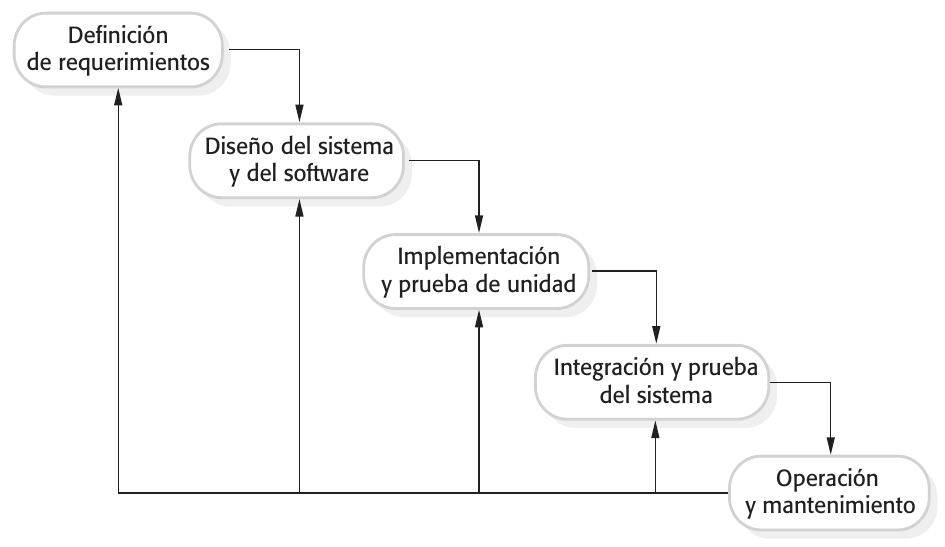
\includegraphics[width=0.95\textwidth]{imagenes/figura2_1.png} % Inserta una imagen
	%		
	%		\begin{flushleft}
	%			\hspace{1.20cm} \textit{Nota.} al pie asociada con esta figura, explicando detalles adicionales. % Nota al pie para esta figura
	%		\end{flushleft}
	%		\vspace{-16pt}
	%		\label{fig:figura2_1} % Etiqueta para referencia cruzada
	%	\end{figure}

	
	
	\section{MARCO LEGAL Y NORMATIVO}
	\subsection{Autoridad de regulación y fiscalización de telecomunicaciones y transportes}
	\subsection{Ley general del transporte}
	\subsection{Reglamento regulatorio de transporte terrestre}


